There are different collections of tracks that could be used to calculate substructure variables. Compared here are tracks that are ghost associated to the ungroomed large-R jet with the collection which is also used for the $\mtas$, see Section \ref{subsec:ObsDef_Proc}, which is ghost association to $k_T$-subjets and $\Delta R$ matching of tracks close to sub-jets.

The distributions showing the number of tracks associated to a calorimeter jet, see the left side of Figure \ref{fig:delta_R}, indicate, that on average around four tracks less are associated to the sub-jets compared to the ungroomed jet. The right side of Figure \ref{fig:delta_R} shows the angular distance $\Delta R$ between the single tracks and the axis of the large-R calorimeter jet. Both distributions are aligned in the lower $\Delta R$ region while the histogram representing the tracks associated to the ungroomed jet shows an enhancement towards larger $\Delta R$. Accordingly, these additional tracks feature an angular separation from the jet axis of more than $0.3$, and are in consequence distributed primarily around the outer regions of the large-R jet. Given the required primary vertex association, it is unlikely that these tracks originate from pile-up. Instead, the origin might be found in final- or initial state radiation. 
\begin{figure}
	\centering
	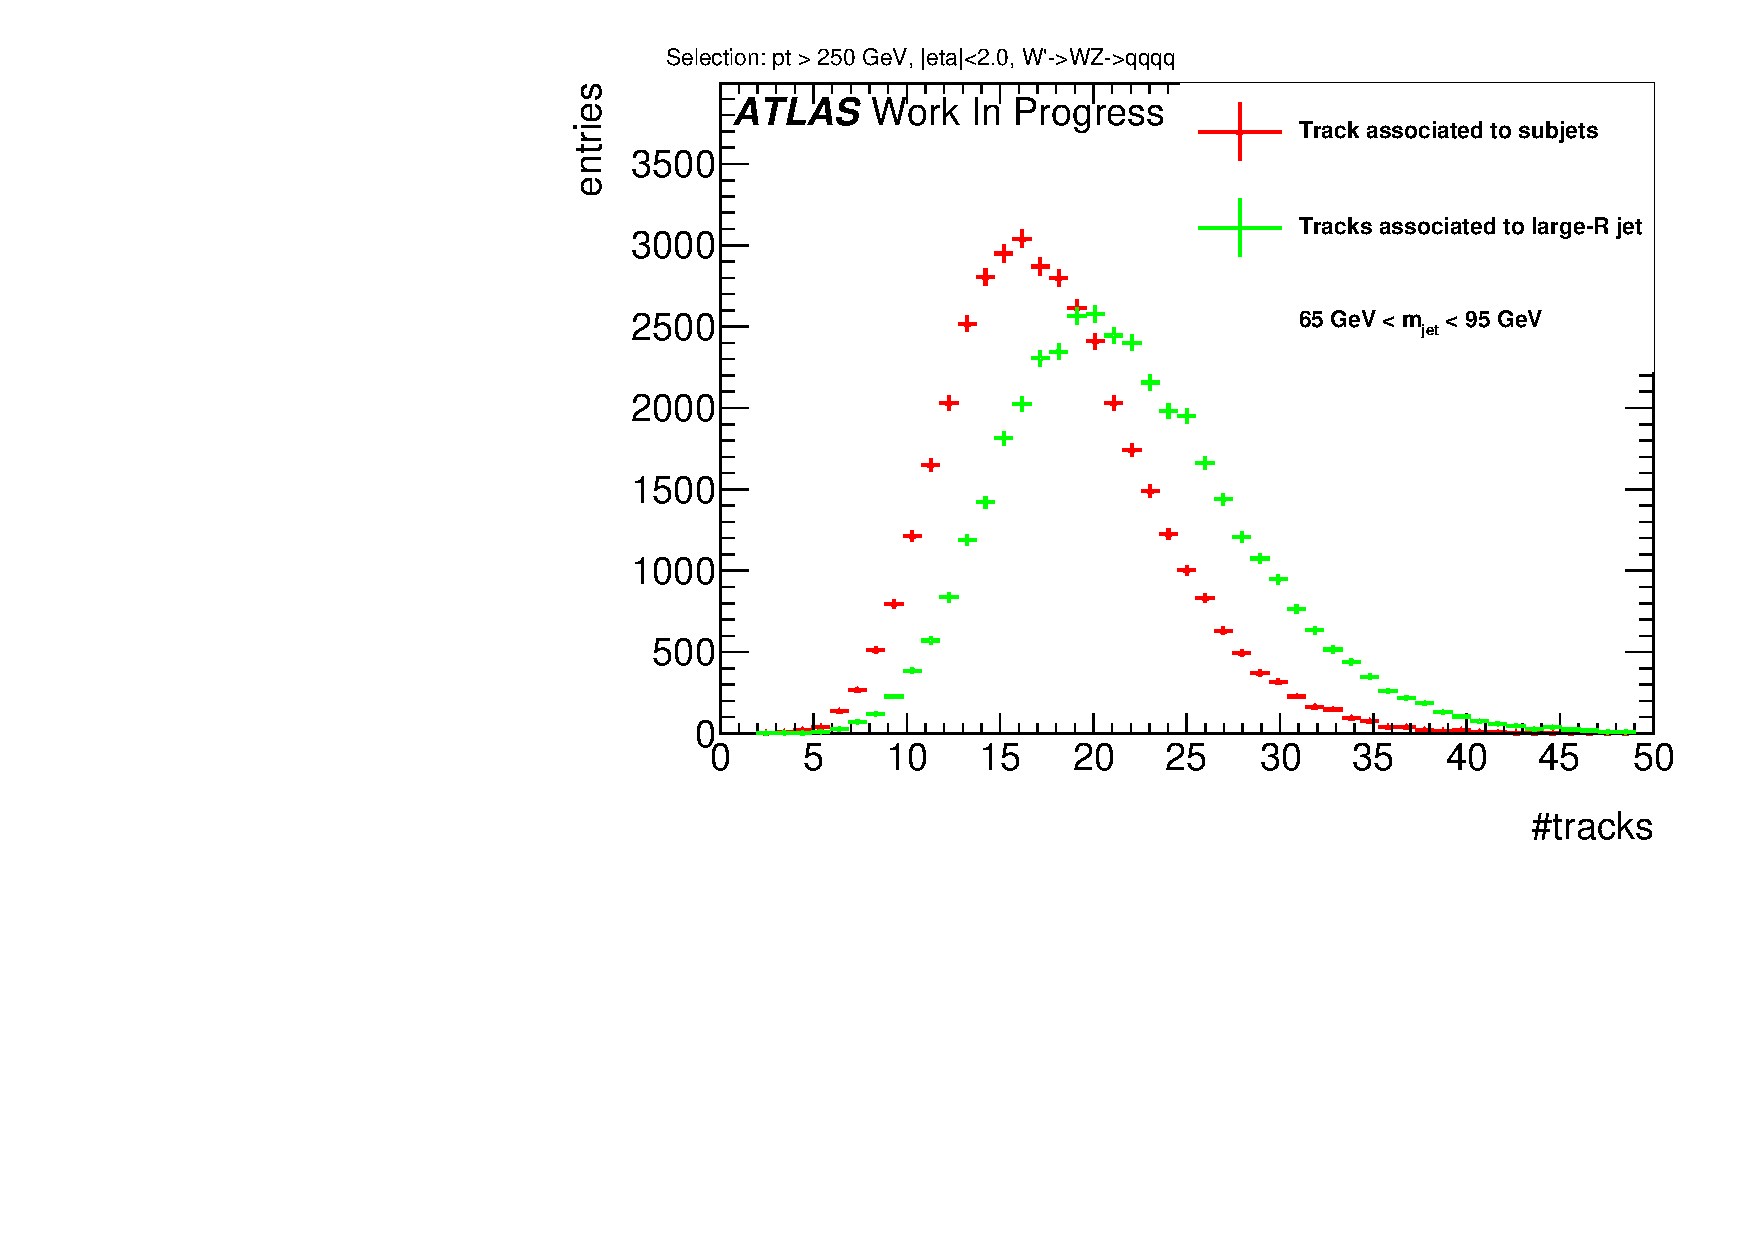
\includegraphics[width=0.45\textwidth]{sascha_input/plots/track_selection/h_customghost_number.pdf} \hspace{1mm}
	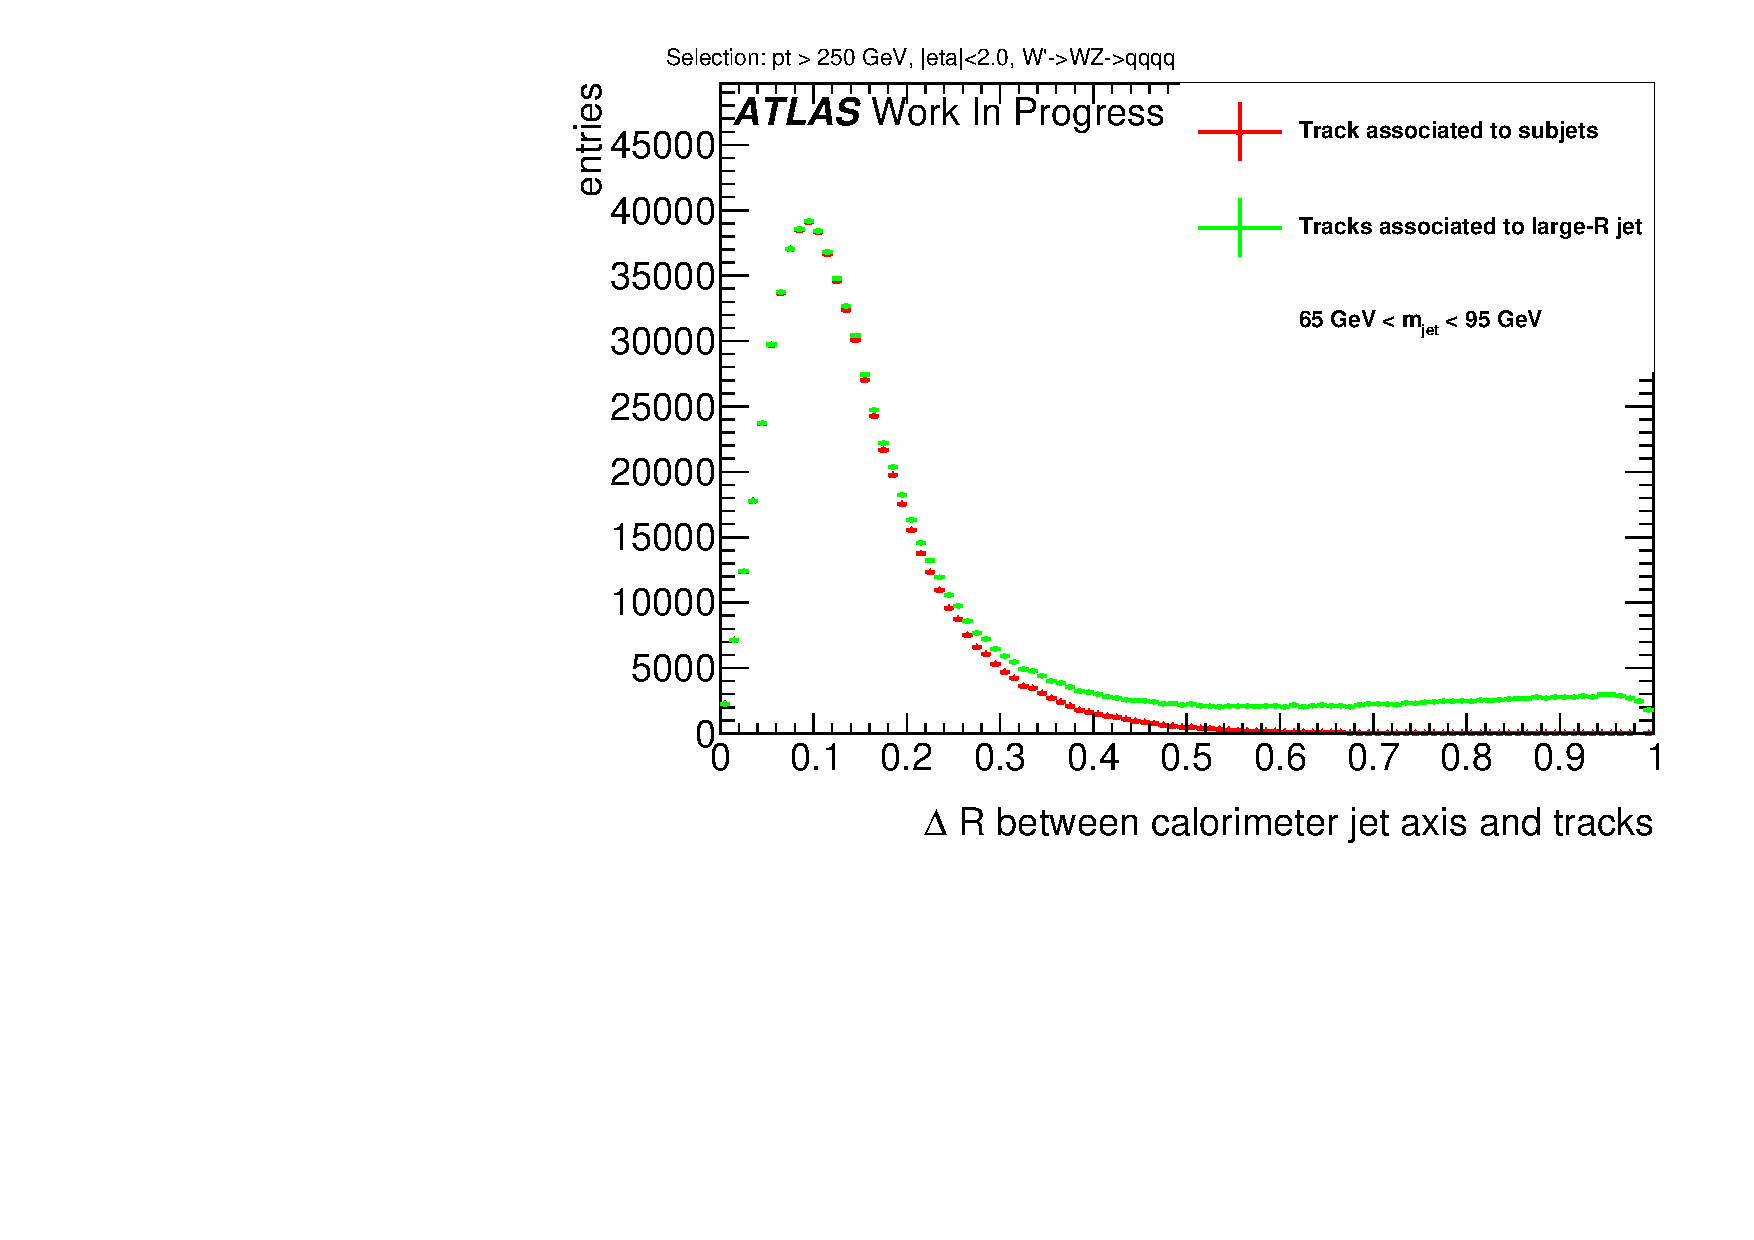
\includegraphics[width=0.45\textwidth]{sascha_input/plots/track_selection/h_customghost_dr.pdf}
\caption{\footnotesize{The number of tracks ghost associated to the large-R jet and to the sub-jets (left) and angular distance of associated tracks to the large-R calorimeter jet axis (right). Signal events were not reweighted at this step.}}\label{fig:delta_R}
\end{figure}


Figure \ref{fig:selection} shows the signal distributions of the C2/D2, and $\tau_{21}$, calculated with both selections of tracks for $W$ boson jets. The large $\Delta R$ to the jet axis of the differing tracks push the substructure variables to higher, more background like values. The broader distributions are a result of the variating nature of these tracks. C2 and D2 are more sensitive to tracks with a large $\Delta R$ to the jet axis, because the angular distance between all pairs and triples of tracks is considered, among tracks on possibly opposite ends of the large-R jet, whereas $\tau_{21}$uses distances to $k_\mathrm{T}$-WTA axes.
\begin{figure}
	\centering
	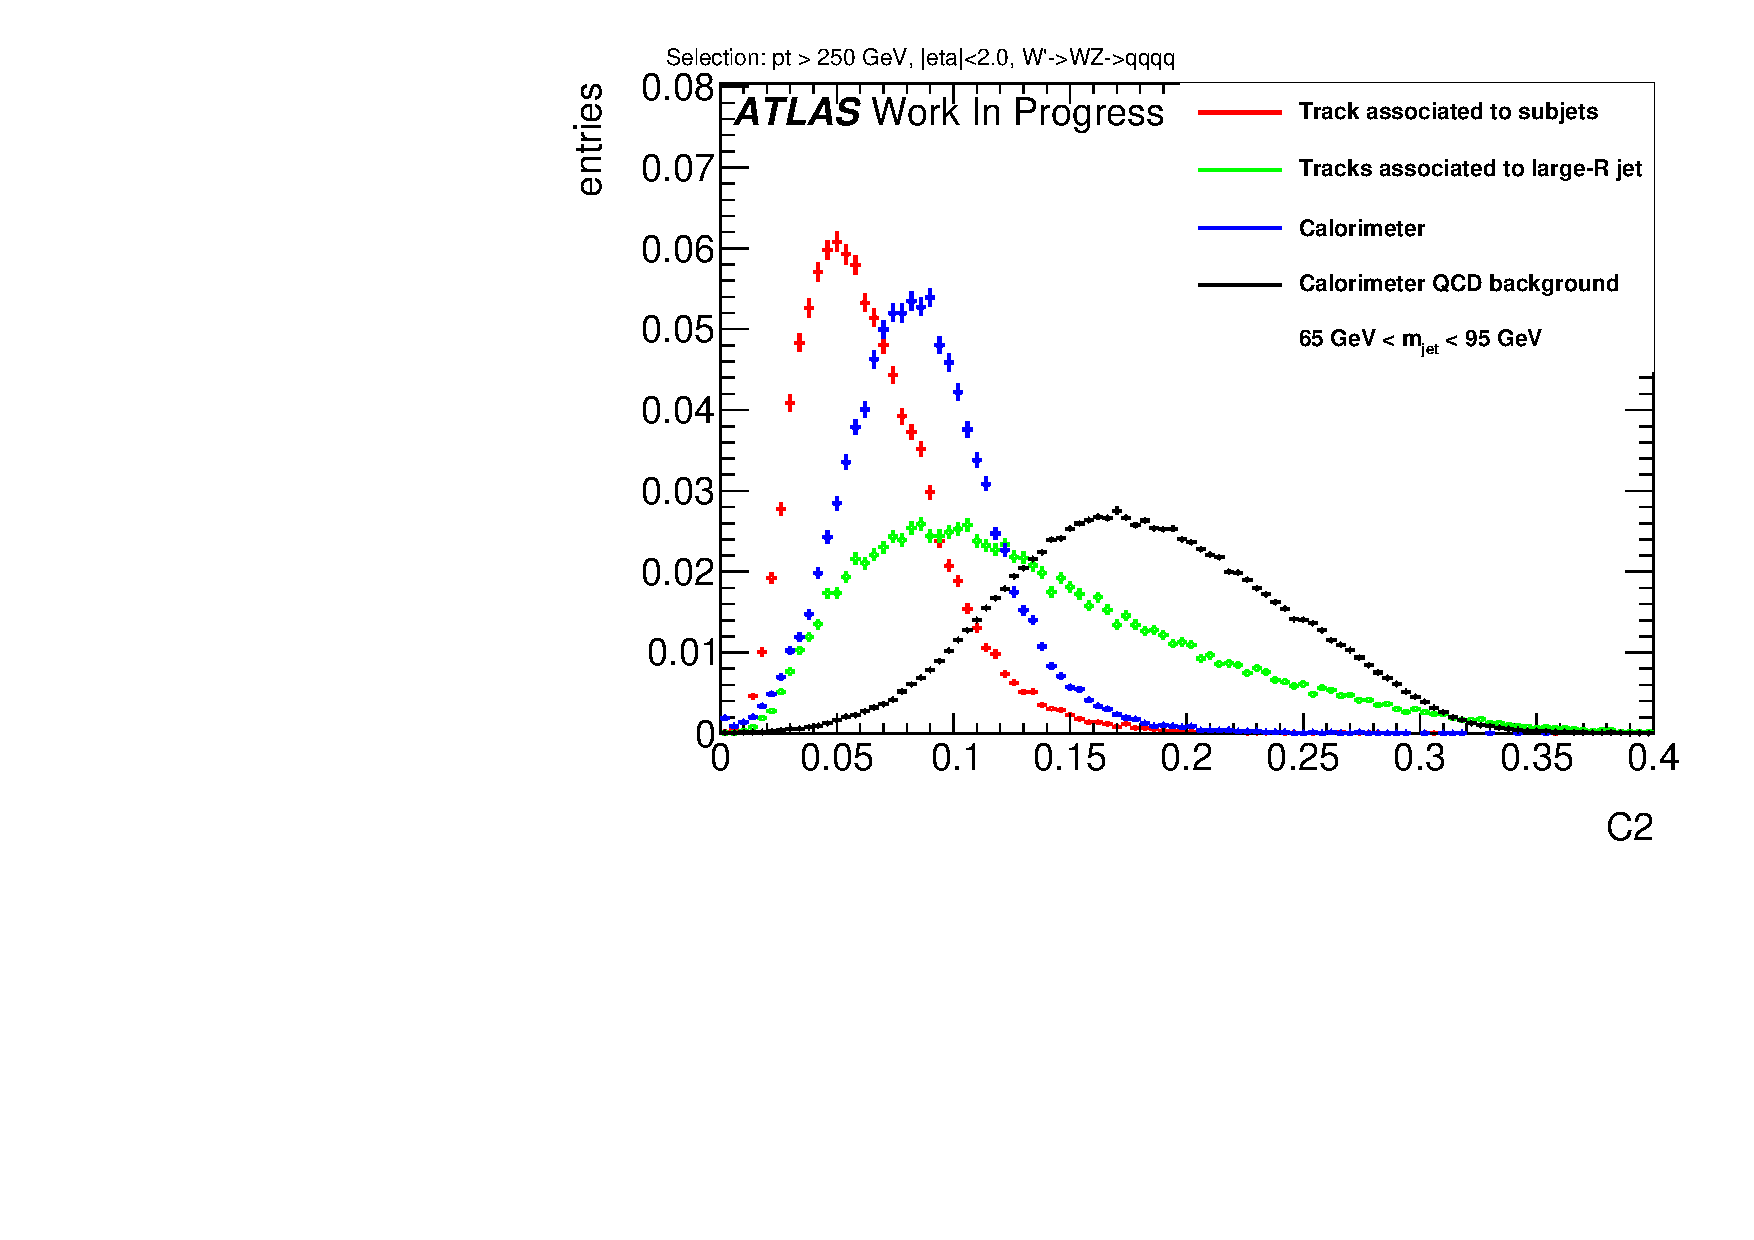
\includegraphics[width=0.3\textwidth]{sascha_input/plots/track_selection/h_ghost_sj_C2.pdf} 
	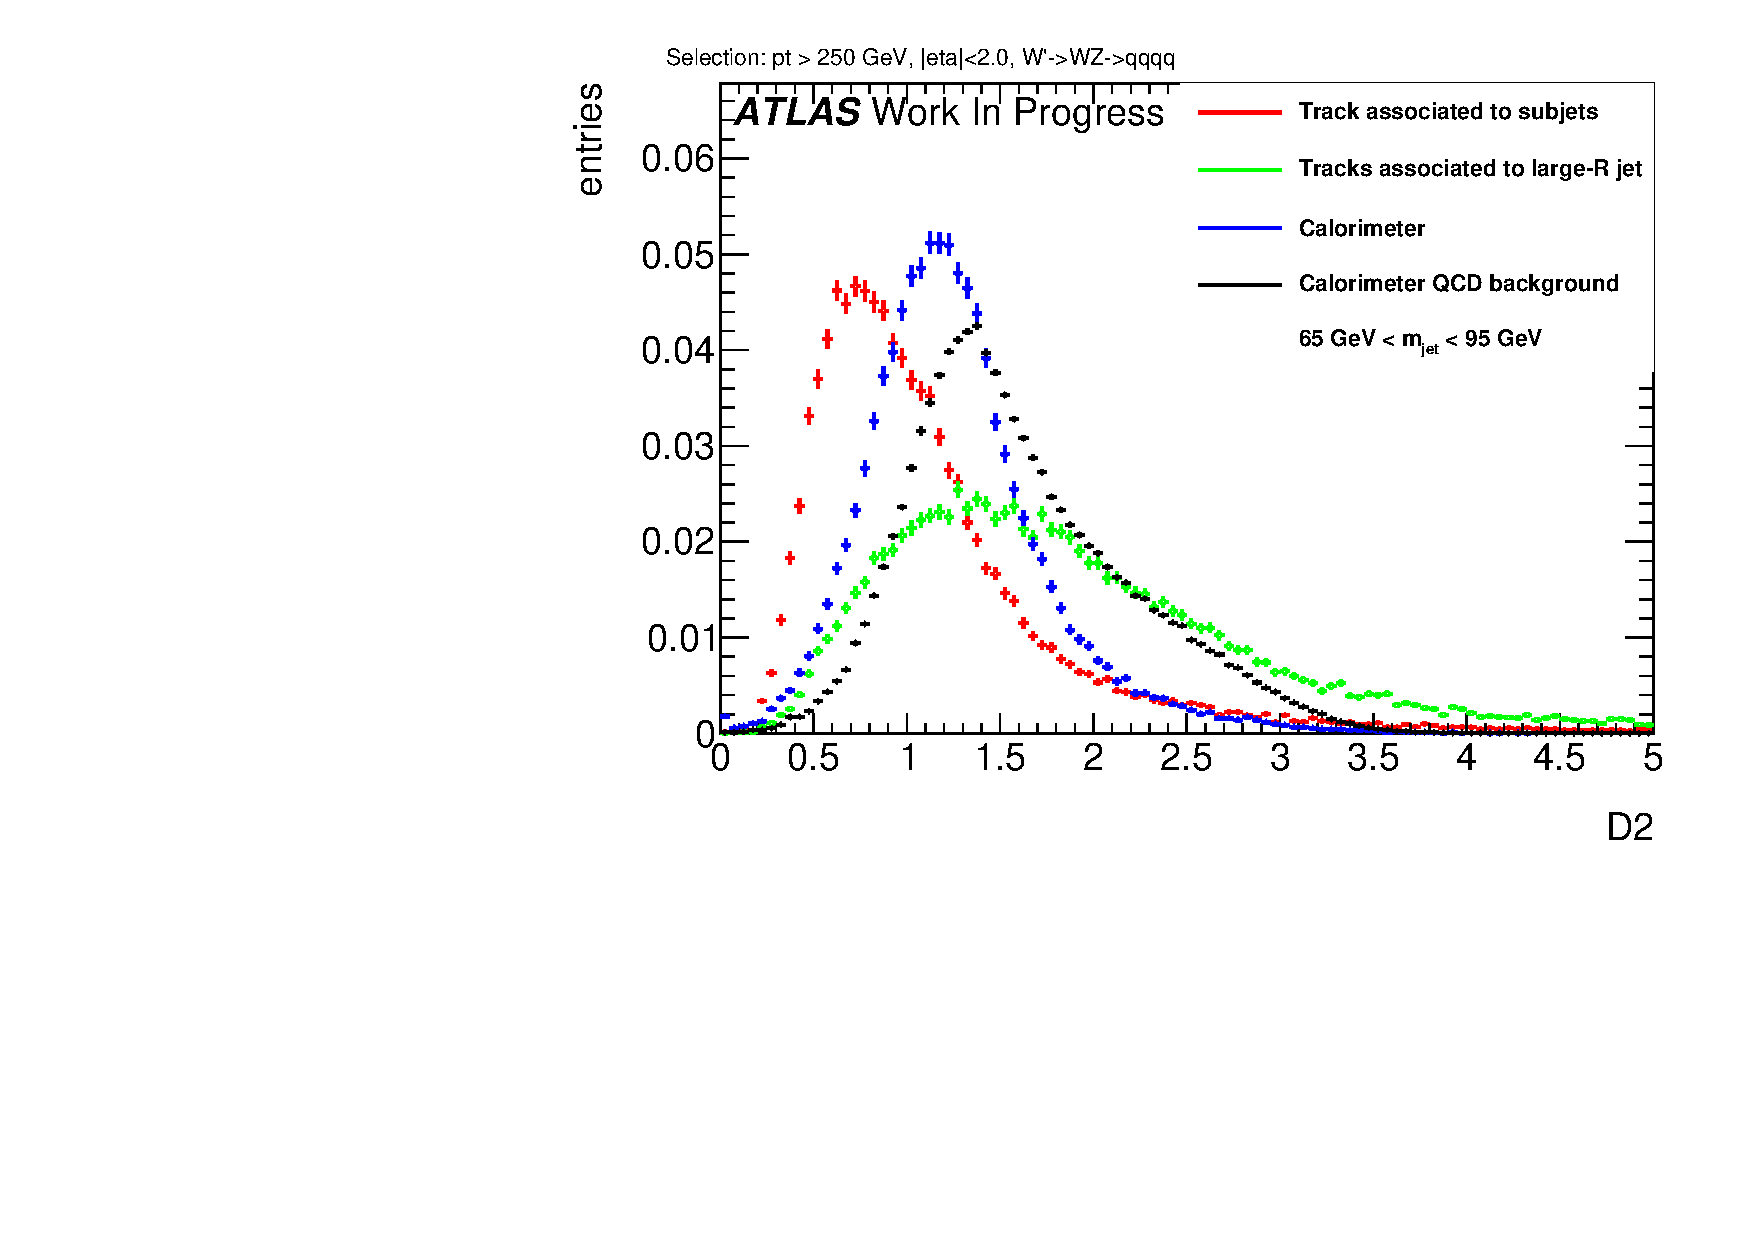
\includegraphics[width=0.3\textwidth]{sascha_input/plots/track_selection/h_ghost_sj_D2.pdf}
	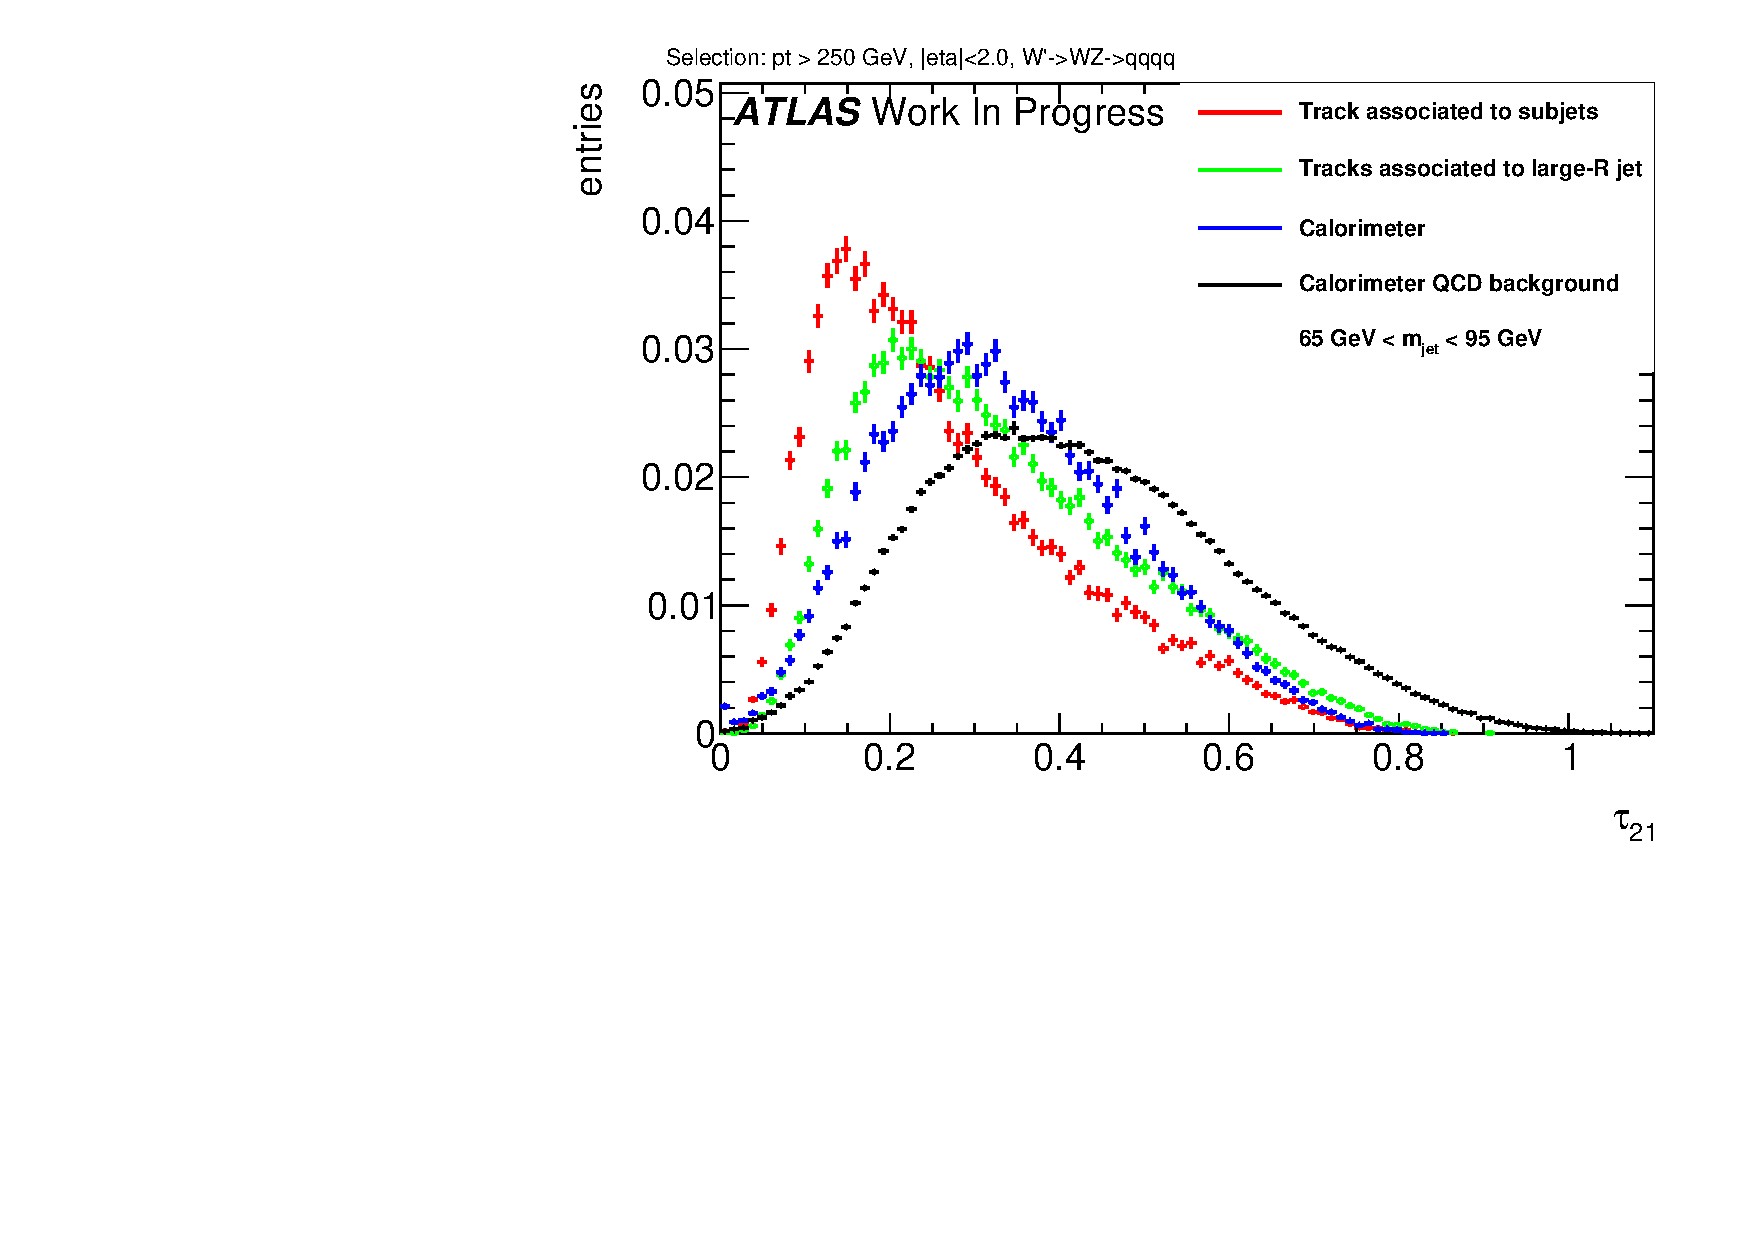
\includegraphics[width=0.3\textwidth]{sascha_input/plots/track_selection/h_ghost_sj_nSub21.pdf}
\caption{\footnotesize{Substructure variables (left) C2, (right) D2 and (below) $\tau_{21}$ calculateated with calorimeter clusters as well as tracks associated to sub-jets and to the large-R jet. Signal events were not reweighted at this step.}}\label{fig:selection}
\end{figure}
For comparison, the signal and background distributions for the variables calculated with calorimeter clusters are shown as well. It is possible to anticipate that the performance of variables calculated with tracks and assisted tracks is not worse than cluster base variables.
In contrast to the previously studied jet mass variable, ratios of ECF(N) and $\tau_N$ are rather energy scale independent and are found to not be as sensitive to the missing neutral fraction with un-assisted tracks.
Starting from this observations, the performance of substructure techniques is compared with the following objects as input:
\begin{itemize}
\item Calorimeter clusters, labeled 'calo'.
\item Tracks selected as described in Section \ref{subsec:ObsDef_Proc}, labeled 'tracks'.
\item The same collection of tracks, assisted as defined in Section \ref{subsec:ta_adapt}, labeled 'TAS'.
\end{itemize}